\documentclass{article}
\usepackage{amsthm}
\usepackage{amsmath, amssymb}
\usepackage[margin=1in]{geometry}
\usepackage{ytableau}
\usepackage{tikz}
\usepackage{graphicx}
\usepackage{hyperref}

\theoremstyle{definition}
\newtheorem{definition}{Definition}
\newtheorem{theorem}{Theorem}

\title{Partitions}
\author{Lewis Reed}
\date{March 2025}

\begin{document}

\maketitle

\section{What is a partition?}

\begin{definition}
    A \textbf{partition} $p(n)$ of a natural number $n$ is a way of writing $n$ as a sum of positive integer parts.
\end{definition}

\noindent
For example, the partitions of 4 look like this:

\[
\begin{aligned}
&4 \\
&3 + 1 \\
&2 + 2 \\
&2 + 1 + 1 \\
&1 + 1 + 1 + 1
\end{aligned}
\]

\noindent
Each number in a partition is called a part. The function $p(n)$ counts the total number of partitions of $n$.
There is no formula for $p(n)$, but Hardy and Ramanujan got very close with their asymptotic formula:

\[
p(n) \sim \frac{1}{4n\sqrt{3}}\exp\left(\pi\sqrt{\frac{2n}{3}}\right)
\]

\noindent
$p(n)$ can be given conditions to produce more specific results, where different results can be compared
and bijections can be drawn.

\begin{theorem}
    $p(n \mid \text{each part is odd}) = p(n \mid \text{each part is distinct})$
\end{theorem}
    
\begin{proof}
Starting with an odd-partition part, ``pair up'' repeated parts and replace them with their double until there are
no repeated parts. Once all repeated parts are paired up, the parts of the partition are all distinct.
\newline For example, consider this partiton of 10 with only odd parts:

\[
5 + 3 + 1 + 1
\]

\noindent
Pair up the two 1s and replace them with 2 to get this new partition:

\[
5 + 3 + 2
\]

\noindent
There are no more repeated parts, so we are now left with a partiton of distinct parts.
\newline Starting with a distinct-part partition, ``split'' any even parts and replace them with their two halves.

\[
5 + 3 + 2
\]

\noindent
Split up the 2 and replace it with two 1s to get this new partition:

\[
5 + 3 + 1 + 1
\]

\noindent
Every odd-part partition uniquely maps to a distinct-part partition and vice versa. This establishes a bijection.
\end{proof}

\newpage

\section{Representing partitions with Young diagrams}

\begin{definition}
    A \textbf{Young diagram} is a diagram used to represent a partition.
\end{definition}

\noindent
It is made up of squares, where each square represents
the value of 1. Each part is represented by a row of squares, with the rows going down in decreasing order.
\newline Here is the Young diagram for the partition of 10, 5 + 3 + 2:

\[
\begin{minipage}{0.3\textwidth}
    \ydiagram[]
        {5,3,2}
\end{minipage}
\begin{minipage}{0.3\textwidth}
    First row: 5 squares \\
    Second row: 3 squares \\
    Third row: 2 squares
\end{minipage}
\]

\noindent
These diagrams can be used to further analyse bijections between different types of partitions.

\begin{theorem}
    $p(n \mid \text{largest part has size $k$}) = p(n \mid \text{has $k$ parts})$
\end{theorem}

\begin{proof}
Consider the \textbf{conjugate} of the previous Young diagram, where the conjugate is the result of
flipping the diagram on its diagonal:

\[
\begin{minipage}{0.3\textwidth}
    \ydiagram[]
        {3,3,2,1,1}
\end{minipage}
\begin{minipage}{0.3\textwidth}
    This represents the partition 3 + 3 + 2 + 1 + 1 which is also a partiton of 10.
\end{minipage}
\]

\noindent
When flipping the diagram, the first row, which is the largest part, becomes the first column, which is the
number of parts. In the previous example, the largest part of the original partition has size 5, and the number of
parts of the conjugate is 5.
\newline Every Young diagram uniquely maps to its conjugate and vice versa. This establishes a bijection.
\end{proof}

\section{Representing partitions with generating functions}

\begin{definition}
    A \textbf{generating function} is a way to represent a sequence of numbers as a power series. 
\end{definition}

\noindent
Since the geometric series identity gives:

\[
\frac{1}{1 - x} = 1 + x + x^2 + x^3 + x^4 + \dots
\]

\noindent
and similarly,

\[
\frac{1}{1 - x^2} = 1 + x^2 + x^4 + x^6 + x^8 + \dots,
\]

\noindent
each term represents including that power of \( x \) any number of times. Extending this pattern, we obtain
the partition generating function:

\[
\prod_{n=1}^{\infty} \frac{1}{1 - x^n}
\]

\noindent
where each factor \( \frac{1}{1 - x^n} \) accounts for the possibility of including the number \( n \) any
number of times in a partition.

\newpage

\noindent
Analysing the first six terms of the partition generating function:

\[
\prod_{n=1}^{\infty} \frac{1}{1 - x^n} = \frac{1}{1-x} \cdot \frac{1}{1-x^2} \cdot \frac{1}{1-x^3} \cdot \frac{1}{1-x^4} \cdot \frac{1}{1-x^5} \cdot \frac{1}{1-x^6} \cdot \dots
\]

\noindent
Each factor can be expanded as follows:

\[
\begin{aligned}
\frac{1}{1-x} &= 1 + x + x^2 + x^3 + x^4 + x^5 + x^6 + \dots \\
\frac{1}{1-x^2} &= 1 + x^2 + x^4 + x^6 + \dots \\
\frac{1}{1-x^3} &= 1 + x^3 + x^6 + \dots \\
\frac{1}{1-x^4} &= 1 + x^4 + \dots \\
\frac{1}{1-x^5} &= 1 + x^5 + \dots \\
\frac{1}{1-x^6} &= 1 + x^6 + \dots
\end{aligned}
\]

\noindent
When we multiply these expansions, the coefficient of $x^6$ in the product will correspond to $p(6)$. To find this coefficient, we need to identify all combinations of terms whose powers sum to 6:

\[
\begin{aligned}
&x^6 \text{ from } \frac{1}{1-x}: \text{ represents the partition } 6 = 1+1+1+1+1+1 \\
&x^4 \cdot x^2 \text{ from } \frac{1}{1-x} \text{ and } \frac{1}{1-x^2}: \text{ represents } 6 = 1+1+1+1+2 \\
&x^2 \cdot x^4 \text{ from } \frac{1}{1-x} \text{ and } \frac{1}{1-x^4}: \text{ represents } 6 = 1+1+4 \\
&x^2 \cdot x^2 \cdot x^2 \text{ from } \frac{1}{1-x^2}: \text{ represents } 6 = 2+2+2 \\
&x^3 \cdot x^3 \text{ from } \frac{1}{1-x^3}: \text{ represents } 6 = 3+3 \\
&x^3 \cdot x^2 \cdot x \text{ from } \frac{1}{1-x^3}, \frac{1}{1-x^2}, \text{ and } \frac{1}{1-x}: \text{ represents } 6 = 3+2+1 \\
&x^3 \cdot x \cdot x \cdot x \text{ from } \frac{1}{1-x^3} \text{ and } \frac{1}{1-x}: \text{ represents } 6 = 3+1+1+1 \\
&x^2 \cdot x^2 \cdot x \cdot x \text{ from } \frac{1}{1-x^2} \text{ and } \frac{1}{1-x}: \text{ represents } 6 = 2+2+1+1 \\
&x^4 \cdot x \cdot x \text{ from } \frac{1}{1-x^4} \text{ and } \frac{1}{1-x}: \text{ represents } 6 = 4+1+1 \\
&x^5 \cdot x \text{ from } \frac{1}{1-x^5} \text{ and } \frac{1}{1-x}: \text{ represents } 6 = 5+1 \\
&x^6 \text{ from } \frac{1}{1-x^6}: \text{ represents the partition } 6 = 6
\end{aligned}
\]

\noindent
Counting these combinations, we find that \( p(6) = 11 \).

\noindent
More generally, if you want to find $p(k)$, you can set the upper limit of the product to $k$ and ignore
any terms in the series with an exponent greater than $k$. So, when $k = 6$, we can expand
$\prod_{n=1}^{6} \frac{1}{1-x^n}$, ignoring the terms where the exponent is greater than 6. We end up with:

\[
(1 + x + x^2 + x^3 + x^4 + x^5 + x^6) \cdot (1 + x^2 + x^4 + x^6) \cdot (1 + x^3 + x^6) \cdot (1 + x^4) \cdot 
(1 + x^5) \cdot (1 + x^6)
\]

\noindent
which, when expanded out, gives us:

\[
1 + x + 2x^2 + 3x^3 + 5x^4 + 7x^5 + 11x^6
\]

\noindent
The coefficient of $x^6$ is 11, which is equal to the number of partitions of 6.

\begin{theorem}
Let $p_2(k)$ be the number of partitions of $k$ where each part is of size at most 2. The generating function for 
$p_2(k)$ is given by the product $\prod_{n=1}^{2} \frac{1}{1-x^n}$.
\end{theorem}

\begin{proof}
To find $p_2(k)$, the number of partitions of $k$ with parts of size at most 2, we only need to expand the first two
terms of the generating function:

\[
\frac{1}{1 - x} \cdot \frac{1}{1 - x^2}
\]

\noindent
Which is equivalent to:

\[
(1 + x + x^2 + x^3 + x^4 + x^5 + x^6 + x^7 + x^8 + \dots) \cdot (1 + x^2 + x^4 + x^6 + x^8 + \dots)
\]

\noindent
When we expand this out, the coefficient of $x^k$ in the product will correspond to $p_2(k)$.
For example, if we want to find $p_2(8)$, we look at the coefficient of $x^8$ in:

\[
1 + x + 2x^2 + 2x^3 + 3x^4 + 3x^5 + 4x^6 + 4x^7 + 5x^8 + \dots
\]

\noindent
Therefore, $p_2(8) = 5$.

\end{proof}

\section{Franklin's involution}

\begin{definition}

Consider a Young diagram of a partition of distinct parts. We can name two regions of the diagram:

\[
\begin{minipage}{0.3\textwidth}
    \begin{ytableau}
        *(white)  & *(white)  & *(white)  & *(white)  & *(white)  & *(blue) \\
        *(white)  & *(white)  & *(white)  & *(white)  & *(blue) \\
        *(green)  & *(green)  & *(green)
    \end{ytableau}
\end{minipage}
\hfill
\begin{minipage}{0.6\textwidth}
    Blue - We call this the \textbf{slope}. \newline
    Green - This is the \textbf{base}, which is simply the smallest part in the partition.
\end{minipage}
\]

\noindent
We can manipulate these regions using a certain method, called \textbf{Franklin's involution}:
\begin{itemize}
    \item If the slope is less than the base, we can ``move'' the slope down below the base to become the new base.
    \item If the slope is greater than or equal to the base, we can ``move'' the base up to become the new slope.
\end{itemize}

\end{definition}

\begin{theorem}
    If Franklin's involution is successful, it will map a partition with either an even number of distinct parts to
    one with an odd number of distinct parts.
\end{theorem}

\begin{proof}

\noindent
For our previous example of the partition of 14, 6 + 5 + 3, which maps a partition with an odd number of parts to
one with an even number of parts:

\[
\begin{minipage}{0.3\textwidth}
    \begin{ytableau}
        *(white)  & *(white)  & *(white)  & *(white)  & *(white)  & *(blue) \\
        *(white)  & *(white)  & *(white)  & *(white)  & *(blue) \\
        *(green)  & *(green)  & *(green)
    \end{ytableau}
\end{minipage}
\hfill
\begin{minipage}{0.3\textwidth}
    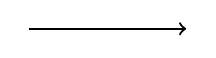
\begin{tikzpicture}
        \draw[thick, ->] (0,0) -- (2,0);
    \end{tikzpicture}
\end{minipage}
\begin{minipage}{0.3\textwidth}
    \begin{ytableau}
        *(white)  & *(white)  & *(white)  & *(white)  & *(white) \\
        *(white)  & *(white)  & *(white)  & *(white)  & \\
        *(green)  & *(green)  & *(green) \\
        *(blue)  & *(blue)
    \end{ytableau}
\end{minipage}
\]

\newpage

\noindent
For this example of the partition of 17, 6 + 5 + 4 + 2, which maps a partition with an even number of parts to
one with an odd number of parts:

\[
\begin{minipage}{0.3\textwidth}
    \begin{ytableau}
        *(white)  & *(white)  & *(white)  & *(white)  & *(white)  & *(blue) \\
        *(white)  & *(white)  & *(white)  & *(white)  & *(blue) \\
        *(white)  & *(white)  & *(white)  & *(blue) \\
        *(green)  & *(green)
    \end{ytableau}
\end{minipage}
\hfill
\begin{minipage}{0.3\textwidth}
    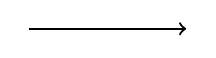
\begin{tikzpicture}
        \draw[thick, ->] (0,0) -- (2,0);
    \end{tikzpicture}
\end{minipage}
\begin{minipage}{0.3\textwidth}
    \begin{ytableau}
        *(white)  & *(white)  & *(white)  & *(white)  & *(white)  & *(blue)  & *(green) \\
        *(white)  & *(white)  & *(white)  & *(white)  & *(blue)  & *(green) \\
        *(white)  & *(white)  & *(white)  & *(blue)
    \end{ytableau}
\end{minipage}
\]

\noindent
The transformation uniquely maps a partition with an even number of parts to one with an odd number of distinct
parts, and vice versa. This establishes a bijection.

\end{proof}

\noindent
For all the partitons of numbers like 10, 9 and 8, every partition with an even number of distinct parts pairs up
exactly with a partition with an odd number of distinct parts. However, for the partitions of a number like 7, there
is a ``leftover'' partition which does not map to any counterpart. This particular example is the partition of 3 + 4,
which looks like this:

\[
\begin{minipage}{0.3\textwidth}
    \ydiagram[]
    {4,3}
\end{minipage}
\hfill
\begin{minipage}{0.3\textwidth}
    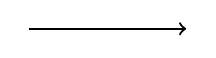
\begin{tikzpicture}
        \draw[thick, ->] (0,0) -- (2,0);
    \end{tikzpicture}
\end{minipage}
\begin{minipage}{0.3\textwidth}
    {\Huge ?}
\end{minipage}
\]

\noindent
The problem with this particular Young diagram is that the slope and base overlap:

\[
\begin{ytableau}
    *(white)  & *(white)  & *(white)  & *(blue) \\
    *(green)  & *(green)  & *(cyan)
\end{ytableau}
\]

\noindent
If you try and perform the involution anyway, you would want to move the slope down to become a new base, since
the slope is less than the base. This would look like this:

\[
\begin{ytableau}
    *(white)  & *(white)  & *(white) \\
    *(green)  & *(green) \\
    *(blue)  & *(cyan)
\end{ytableau}
\]

\noindent
Since this involves moving a part of the old base, this is creates the partition 3 + 2 + 2, which is no
longer a partition of distinct parts. This means the involution fails. \par

\vspace{10pt}

\noindent
Another example of where there is a leftover partition which does not map to any counterpart is the partitions of 12.
The particular diagram where the involution fails is for the partition 5 + 4 + 3, which looks like this:

\[
\begin{minipage}{0.3\textwidth}
    \ydiagram[]
    {5,4,3}
\end{minipage}
\hfill
\begin{minipage}{0.3\textwidth}
    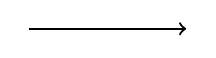
\begin{tikzpicture}
        \draw[thick, ->] (0,0) -- (2,0);
    \end{tikzpicture}
\end{minipage}
\begin{minipage}{0.3\textwidth}
    {\Huge ?}
\end{minipage}
\]

\noindent
In this case the slope and base also overlap:

\[
\begin{ytableau}
    *(white)  & *(white)  & *(white)  & *(white)  & *(blue) \\
    *(white)  & *(white)  & *(white)  & *(blue) \\
    *(green)  & *(green)  & *(cyan)
\end{ytableau}
\]

\newpage

\noindent
Trying to perform the involution anyway, means you would want to move the base up to become the new slope, since
the slope is equal to the base. This would look like this:

\[
\begin{minipage}{0.25\textwidth}
    \begin{ytableau}
        *(white)  & *(white)  & *(white)  & *(white)  & *(blue)  & *(green) \\
        *(white)  & *(white)  & *(white)  & *(blue)  & *(green) \\
    \end{ytableau}
\end{minipage}
\hfill
\begin{minipage}{0.25\textwidth}
    \begin{ytableau}
        *(cyan)
    \end{ytableau}
\end{minipage}
\hfill
\begin{minipage}{0.25\textwidth}
    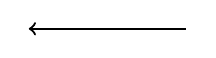
\begin{tikzpicture}
        \draw[thick, <-] (0,0) -- (2,0);
    \end{tikzpicture}
\end{minipage}
\hfill
\begin{minipage}{0.25\textwidth}
    \fbox{
        \parbox{\textwidth}{\centering No rows left \\ in the slope for \\ this square}
    }
\end{minipage}
\]

\noindent
Since this involves moving a part of the old slope, there are less rows than the new slope, leaving one square free.
This means the involution fails. \par

\vspace{10pt}

\noindent
There is a pattern for which numbers have partitons where Franklin's involution fails. The numbers 7 and 12 are
examples of generalised pentagonal numbers.

\section{Pentagonal number theorem}

\begin{definition}
The set of \textbf{generalised pentagonal numbers} is an extended version of the set of pentagonal numbers:

\begin{figure}[h]
    \centering
    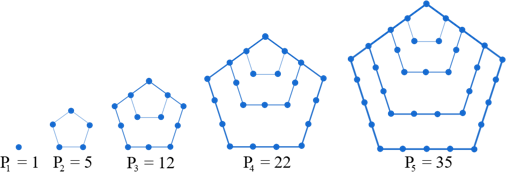
\includegraphics[width=0.5\textwidth]{pentagonal_numbers.png}
    \caption{Pentagonal numbers. Source: \url{https://www.math.net/pentagonal-number}, March 2025.}
\end{figure}

\end{definition}

\noindent
Where a pentagonal number $P_k$ follows:

\[
P_k = \frac{k(3k - 1)}{2} \text{for $k = 0, 1, 2, 3, \dots$}
\]

\noindent
And a generalised pentagonal number follows:

\[
P_k = \frac{k(3k - 1)}{2} \text{for $k = 0, \pm 1, \pm 2, \pm 3, \dots$}
\]

\begin{theorem}
The theorem states that:

\[
\prod_{n=1}^{\infty} (1 - x^n) = \sum_{-\infty}^{\infty} (-1)^k x^{\frac{k(3k-1)}{2}}
\]

\noindent
This means that if we expand the left-hand side, we get a series with plus and minus signs, and the powers of $x$
in the series are pentagonal numbers.

\end{theorem}

\begin{proof}

Considering the cases where Franklin's involution fails, we can use this to derive:

\[
p_e(n) = p_o(n) + \epsilon(n)
\]

\noindent
Where $p_e(n)$ and $p_o(n)$ are the number of partitions with an even or odd number of distinct parts, respectively,
and:

\[
\epsilon(n) = 
    \begin{cases}
        (-1)^k & \text{if } n = \frac{k(3k-1)}{2} \\
        0 & \text{if anything else}
    \end{cases}
\]

\noindent
We know this is true because for most $n$, the number of partitions with an even number of distinct parts is the
same as the number of partitions with an odd number of distinct parts. However, when $n$ is a pentagonal number,
Franklin's involution fails in exactly one case, leading to an extra even or odd partition. It is exactly one case
because for a given $n$ that is a generalised pentagonal number, there is exactly one way to form the Young diagram
where the overlap occurs. \par

\vspace{10pt}

\noindent
Reframing this in the form of a generating function:

\[
\sum_{n=0}^{\infty} (p_e(n) - p_o(n)) \cdot x^n
\]

\noindent
From the previous identity, we know this is equal to:

\[
\sum_{n=0}^{\infty} \epsilon(n) \cdot x^n
\]

\noindent
This can also be written as:

\[
\sum_{-\infty}^{\infty} (-1)^k x^{\frac{k(3k-1)}{2}} = (1 - x)(1 - x^2)(1 - x^3)(1 - x^4)(1 - x^5)\dots
\]

\noindent
We know this because the product \((1-x)(1-x^2)(1-x^3)\cdots\) expands to a sum where almost every term cancels out
due to the pairing, except for the special cases. This is why the sum ends up being

\[
\sum_{-\infty}^{\infty} (-1)^k x^{\frac{k(3k-1)}{2}},
\]

\noindent
which is exactly what the pentagonal number theorem states.

\end{proof}

\noindent
From this, we can see:

\[
\prod_{n=1}^{\infty} (1 - x^n) = 1 - x - x^2 + x^5 + x^7 - x^{12} - \dots
\]

\section{Euler's recurrence relation}

\begin{definition}
\textbf{Euler’s recurrence relation} expresses the partition function \( p(n) \) in terms of previous
values using contributions from generalized pentagonal numbers. It is given by:

\[
p(n) = p(n-1) + p(n-2) - p(n-5) - p(n-7) + \dots
\]

\noindent
where the terms correspond to the generalized pentagonal numbers \( g_k = \frac{k(3k-1)}{2} \) for
\( k = \pm 1, \pm 2, \pm 3, \dots \), and the signs alternate based on \( k \).

\end{definition}

\begin{theorem}
For all \( n \geq 1 \),

\[
p(n) = \sum_{k \neq 0} (-1)^{k+1} p(n - P_k)
\]

\noindent
where \( P_k = \frac{k(3k-1)}{2} \) are the generalized pentagonal numbers, and the sum runs over all
nonzero integers \( k \).

\end{theorem}

\begin{proof}

\noindent
Recall the generating function for $p(n)$:

\[
\sum_{n=0}^{\infty} p(n)x^n = \prod_{j=1}^{\infty} \frac{1}{1-x^j}
\]

\noindent
We also now know, from the pentagonal number theorem, that:

\[
\prod_{j=1}^{\infty} (1 - x^j) = 1 - x - x^2 + x^5 + x^7 - x^{12} - \dots
\]

\noindent
Using what we now know, we can rewrite the partition generating function:

\[
\begin{aligned}
\sum_{n=0}^{\infty} p(n)x^n &= \prod_{j=1}^{\infty} \frac{1}{1-x^j} \\
&= \frac{1}{\prod_{j=1}^{\infty} (1 - x^j)} \\
&= \frac{1}{1 - x - x^2 + x^5 + x^7 - x^{12} - \dots}
\end{aligned}
\]

\noindent
Therefore, we can write:

\[
(\sum_{n=0}^{\infty} p(n)x^n) \cdot (1 - x - x^2 + x^5 + x^7 - x^{12} - \dots) = 1
\]

\noindent
Since this is simply the generating function multiplied by 1 over itself. We can expand this expression to get:

\[
\sum_{n=0}^{\infty} p(n)x^n - \sum_{n=1}^{\infty} p(n - 1)x^n - \sum_{n=2}^{\infty} p(n - 2)x^n -
\sum_{n=5}^{\infty} p(n - 5)x^n - \sum_{n=7}^{\infty} p(n - 7)x^n - \dots = 1
\]

\noindent
Since we know the sum is 1, the coefficients of the $x^n$ terms must equal 0. Therefore:

\[
p(n) - p(n-1) - p(n - 2) + p(n - 5) + p(n - 7) - \dots = 0
\]

\noindent
Which we can rearrange to be:

\[
p(n) = p(n-1) + p(n - 2) - p(n - 5) - p(n - 7) + \dots
\]

\noindent
This is exactly Euler's recurrence relation.

\end{proof}

\end{document}